In this section we present results obtained with DMF$^2$RG.  We use an interpolative cutoff: $[G_0^\Lambda(\mathbf{k},\omega)]^{-1} = (1-\Lambda)[G_0(\mathbf{k},\omega)]^{-1}+\Lambda \mathcal{G}_{\mathrm{AIM}}(\omega)$, ($\mathcal{G}_{\mathrm{AIM}}$ is the propagator of the DMFT self-consistent Anderson impurity model associated with the lattice under consideration. The initial condition for the vertex and the self-energy is per se frequency dependent. 
Apart for this, the implementation is equivalent to the one used in fRG, i.e., same frequency and momentum treatments. 
The self-energy is however better-behaved, compared to the fRG situation: we speculate that this is a consequence of the fact that the flow only has to compute the deviation from the DMFT self-energy. Hence the results with the self energy feedback of this section are numerically more stable.  

The results presented here are (in the usual fRG units) for $U=6.8t$, $T=0.08t$, filling $n=0.85$, and next neighbors hopping $t'=-0.3$.  
\begin{figure}
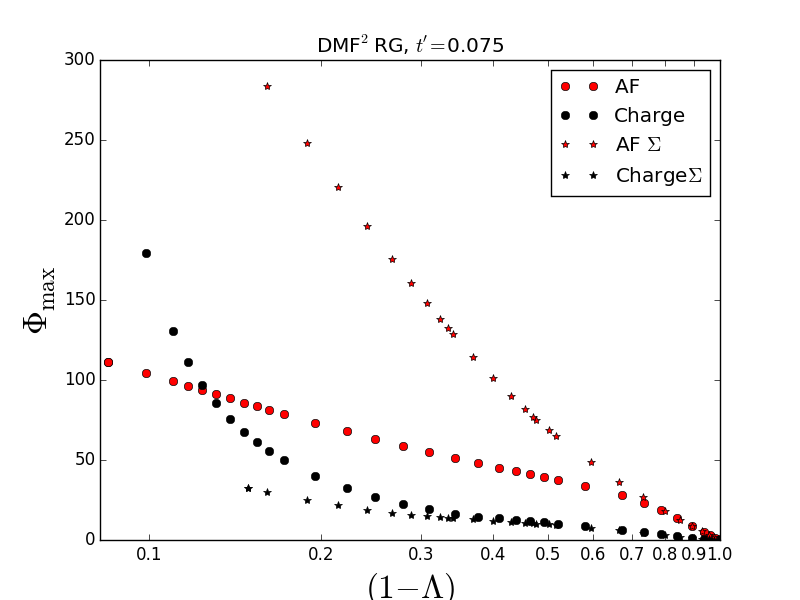
\includegraphics[scale=0.70]{images/dmf2rglam.png}
\caption{Flow of the maximum absolute value of the real part of the magnetic and charge channel in DMF$^2$RG, with and without self-energy feedback.} \label{dmf2rglam}
\end{figure}

\begin{figure}
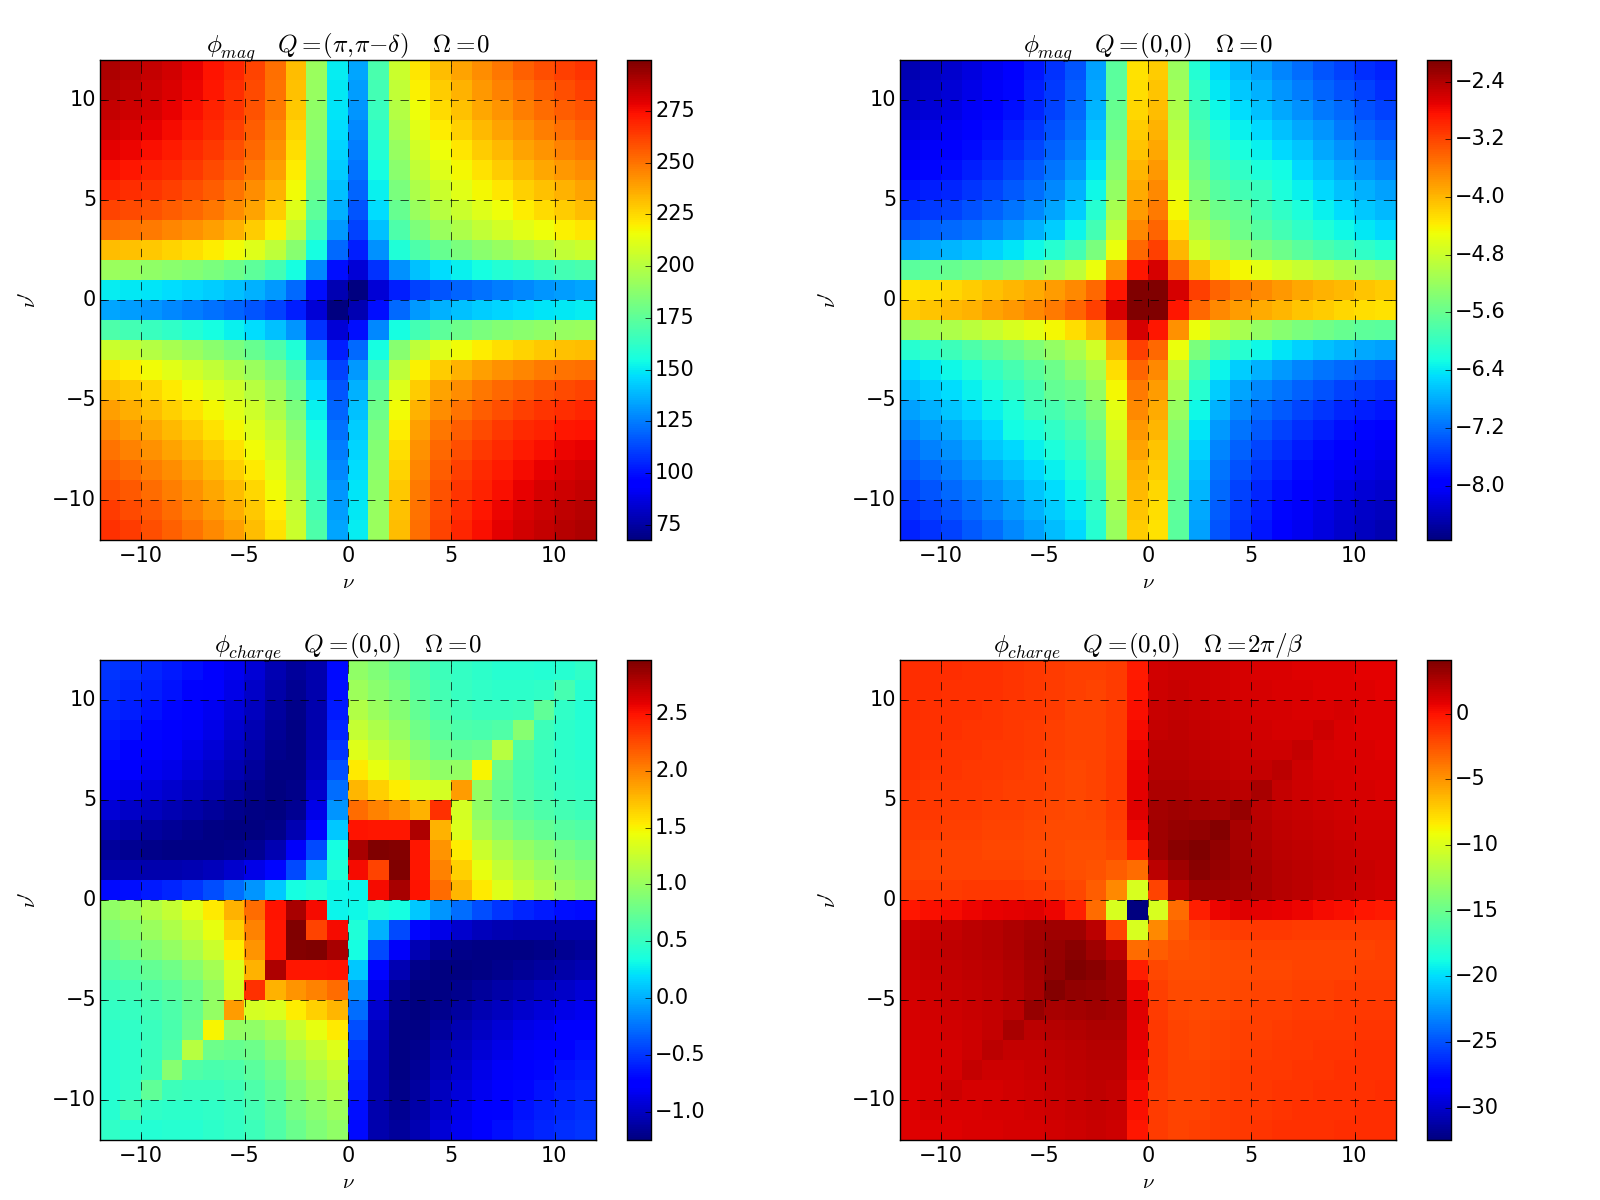
\includegraphics[scale=0.25]{images/Merged_dmf2rg_se.png}
\caption{Frequency dependence of the $\Phi$'s in DMF$^2$RG with self-energy feedback.} \label{dmf2rfreq}
\end{figure}

\subparagraph{Results} 
\begin{itemize}

\item The charge channel instability is present also in DMF$^2$RG, even if the DMFT self energy broadens the Fermi surface, see Fig. \ref{dmf2rflam}.  

\item At large coupling, and without self-energy feedback, we have observed a divergence of the charge channel for any parameter set studied (excluding the case of particle-hole symmetry)$\rightarrow$ up to now the charge-channel divergence is the bottleneck of DMF$^2$RG;  

\item While in fRG the charge divergence seemed to be associated to a crossover from iAF to FM, the charge channel divergence arises in a  AF dominated region;
 
\item The richer frequency structure of the magnetic channel (as compared to the one of fRG) can be understood in terms of ladder diagrams: the same frequency structure arises from Bethe-Salpeter-like equations using the DMFT irreducible vertex, see Fig. \ref{dmf2rfreq}

\end{itemize}

\begin{figure}
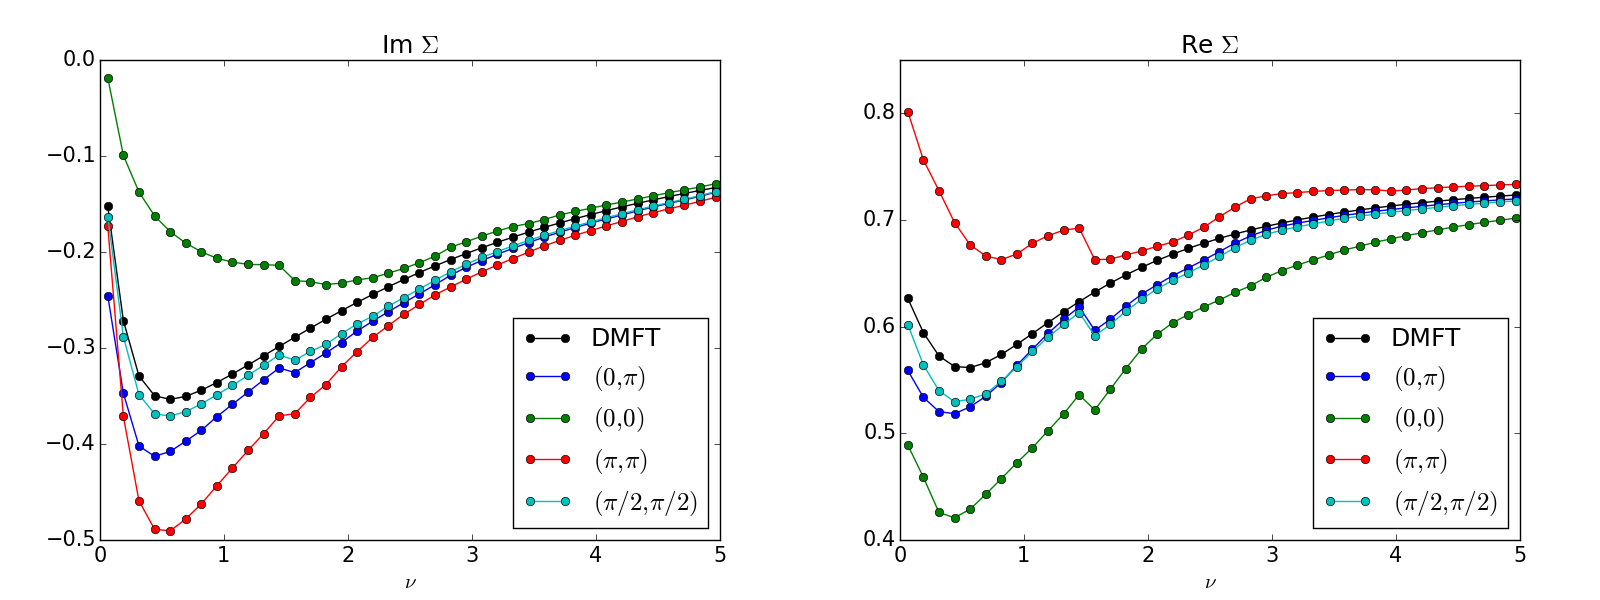
\includegraphics[scale=0.25]{images/Merged_dmf2rg_se_freq.png}
\caption{DMFT and DMF$^2$RG self energy at the critical scale.} \label{dmf2self}
\end{figure}



\subparagraph{Self energy feedback}
\begin{itemize}
\item The self energy suppresses the charge-channel (see Fig. \ref{dmf2rglam}), while being less effective on the AF vertex; 
\item 	The AF channel flow is unusual: it grows towards large coupling value, without "exploding" for a well defined value of critical $\Lambda$. This effect can be possibly due either to the the "interpolative" cutoff used or to a feedback effect of the self energy that avoids a sudden "explosion" of the vertex. 
\item The momentum dependence of the self-energy is relatively modest: there are deviations from the local DMFT self energy, but the self energy remains Fermi-liquid like in all the BZ, see Fig. \ref{dmf2self} Why such a small change of $\Sigma$ has such a large consequence on the flow? 

\item \textbf{TODO}: Study of the effect of the momentum dependence of the self-energy on the bubble. Compare $\nu$ dependent bubble at a given cutoff with and without self energy feedback. Subtract then local bubble to be more consistent. 
\item \textbf{TODO}: How is the ferromagnetism affected by the self energy? Is it a general effect that the self energy suppress the bubble more at $0,0$ than at $\pi,\pi$i? 
\end{itemize} 

